% !TEX root = ../slides.tex
%%%%%%%%%%%%%%%%%%%%%%%%%%%%%%%%%%%%%%%%%%%%%%%%%%%%%%%%%%%%%%%%%%%%%%%%%%%%%%%%
% Session 6: Finite elements in d = 1
%%%%%%%%%%%%%%%%%%%%%%%%%%%%%%%%%%%%%%%%%%%%%%%%%%%%%%%%%%%%%%%%%%%%%%%%%%%%%%%%

\session{session06}{The finite-elements method}{Finite elements in \texorpdfstring{$d=1$}{d=1}}
{Chapter 3}
{\notebook{lectures/finite-elements/d-1/Hermite}{Hermite.ipynb},
    \notebook{lectures/finite-elements/d-1/Bsplines}{Bsplines.ipynb}}
{3.1}

\begin{frame}{Plan for today}
    \begin{enumerate}
        \item Linear and Lagrange elements; computing integrals with Gaussian quadrature.
        \item Hermite cubics: a $C^1$ (hence $H^2$) finite-element space.
        \item Implementation: reference matrices and assembly.
        \item B-splines: maximal smoothness with small support.
    \end{enumerate}
    \bigskip
    \begin{center}
        \begin{tabular}{@{}lccc@{}}
            \toprule
            Element         & Shape functions on $K$ & Global smoothness & Error in $H^1$ \\
            \midrule
            Linear          & $\R_1[x]$              & $C^0$             & $O(h)$         \\
            Lagrange        & $\R_N[x]$              & $C^0$             & $O(h^N)$       \\
            Hermite cubics  & $\R_3[x]$              & $C^1$             & $O(h^3)$       \\
            B-splines       & $\R_p[x]$              & $C^{p-1}$         & $O(h^p)$       \\
            \bottomrule
        \end{tabular}
    \end{center}
    {\small (rates for smooth enough solutions)}
\end{frame}

\begin{frame}{Linear elements revisited}
    \begin{itemize}
        \item Hat functions; error estimated by hand in Session 2.
        \item With Bramble--Hilbert (Session 4): $E(v) = v - \big(v(0) + (v(1) - v(0))x\big)$ vanishes on $\R_1[x]$, so
              \[
                  \|E(v)\|_{H^1(0,1)} \le C \|v''\|_{L^2(0,1)} .
              \]
              This argument also works for $d > 1$.
    \end{itemize}
    \begin{remark}[Matrices via Gaussian quadrature]
        Constant-coefficient stiffness and mass matrices need $\int_{x_k}^{x_{k+1}} \varphi_j^{(r)} \varphi_i^{(s)}$ with $r,s \in \{0,1\}$: polynomials of degree $\le 2$.
        The $2$-point Gauss rule is exact for degree $3$: for $P \in \R_3[x]$,
        \[
            \int_{x_k}^{x_{k+1}} P(x) \diff x = \frac{x_{k+1} - x_k}{2}\Big( Q\big(-\tfrac{1}{\sqrt3}\big) + Q\big(\tfrac{1}{\sqrt 3}\big) \Big),
        \]
        where $Q(\xi) = P\big(\frac{x_{k+1} - x_k}{2}\xi + \frac{x_{k+1} + x_k}{2}\big)$.
    \end{remark}
\end{frame}

\begin{frame}{Lagrange elements}
    $K = (0,1)$, \ $\mathcal P = \R_N[x]$, \ equi-distant nodes $x_i = \frac{i-1}{N}$, \ $N_i(v) = v(x_i)$, \ $i = 1, \dots, N+1$.
    \medskip

    Nodal basis: the Lagrange polynomials
    \[
        \psi_i(x) = \prod_{j \ne i} \frac{x - x_j}{x_i - x_j}.
    \]
    \begin{itemize}
        \item Glueing is continuous (the end points are nodes): $H^1$-type spaces.
        \item Interpolation error: for $u \in C^{N+1}([0,1])$ there is $\xi(x) \in (0,1)$ with
              \[
                  u(x) - \mathcal I_K u(x) = \frac{u^{(N+1)}(\xi(x))}{(N+1)!} \prod_{i=1}^{N+1} (x - x_i).
              \]
        \item Very good for $N$ fixed and $h \to 0$.
        \item Dangerous for $N \to \infty$ with equi-distant nodes: \alert{Runge's phenomenon} (Session 10).
    \end{itemize}
\end{frame}

\begin{frame}{Hermite cubics}
    \small
    Goal: a \alert{$C^1$} global interpolant (needed e.g.\ for fourth-order problems posed in $H^2$).
    \begin{columns}[c]
        \begin{column}{.55\textwidth}
            On $K = (a,b)$: $\mathcal P = \R_3[x]$,
            \begin{align*}
                N_1(v) & = v(a),  & N_2(v) & = v(b),  \\
                N_3(v) & = v'(a), & N_4(v) & = v'(b).
            \end{align*}
            Nodal basis, with $\xi = \frac{x - a}{b - a}$:
            \begin{align*}
                \psi_1 & = \theta_0(\xi),        & \psi_2 & = \theta_1(\xi),        \\
                \psi_3 & = (b-a)\theta_2(\xi),   & \psi_4 & = (b-a)\theta_3(\xi),
            \end{align*}
            where $\theta_0, \dots, \theta_3$ is the nodal basis on $(0,1)$ (Session 4).
        \end{column}
        \begin{column}{.42\textwidth}
            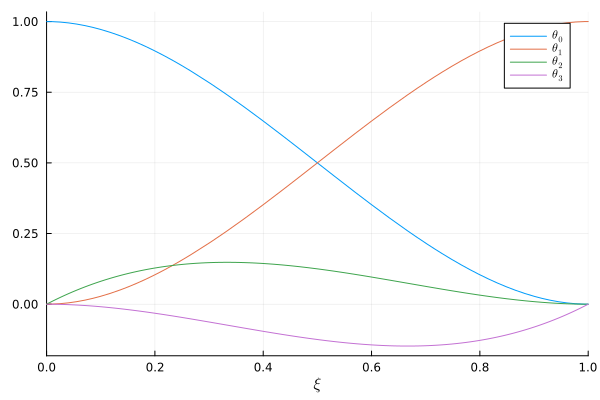
\includegraphics[width=\textwidth]{../../lectures/finite-elements/d-1/Hermite/Hermite_reference_element.png}
        \end{column}
    \end{columns}
    \medskip
    \textbf{Local error.} After rescaling, the factors $(b-a)$ cancel, so (Bramble--Hilbert, $m = 4$):
    \[
        [v - \mathcal I_K v]_{W^{j,p}(K)} \le C h_K^{4-j} [v]_{W^{4,p}(K)}, \qquad j = 0, \dots, 4.
    \]
\end{frame}

\begin{frame}{Global $C^1$ basis}
    Mesh $a = x_0 < x_1 < \cdots < x_{N+1} = b$. Two basis functions per node:
    \[
        v_i(x_j) = \delta_{ij},\quad v_i'(x_j) = 0, \qquad w_i(x_j) = 0, \quad w_i'(x_j) = \delta_{ij}.
    \]
    \begin{columns}[c]
        \begin{column}{.5\textwidth}
            \[
                v_i(x) =
                \begin{cases}
                    \theta_1\big(\frac{x - x_{i-1}}{x_i - x_{i-1}}\big) & x \in [x_{i-1}, x_i), \\[.5ex]
                    \theta_0\big(\frac{x - x_i}{x_{i+1} - x_i}\big)     & x \in [x_i, x_{i+1}), \\[.5ex]
                    0                                                   & \text{otherwise,}
                \end{cases}
            \]
            and similarly $w_i$, using $(x_i - x_{i-1})\theta_3$ and $(x_{i+1} - x_i)\theta_2$.
        \end{column}
        \begin{column}{.48\textwidth}
            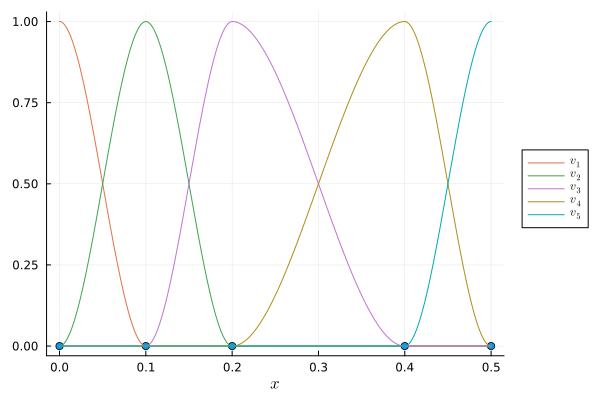
\includegraphics[width=.49\textwidth]{../../lectures/finite-elements/d-1/Hermite/Hermite_interval_v.png}
            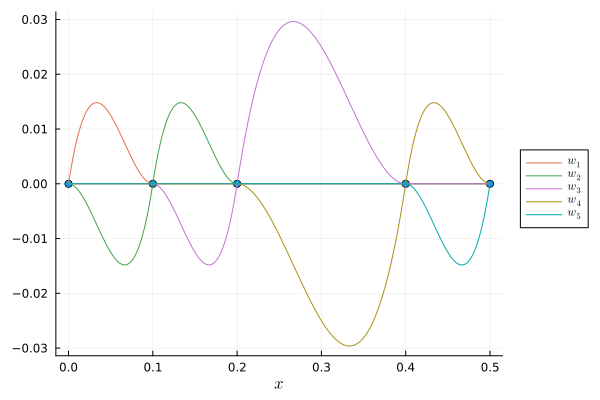
\includegraphics[width=.49\textwidth]{../../lectures/finite-elements/d-1/Hermite/Hermite_interval_w.png}
        \end{column}
    \end{columns}
    \medskip
    Global interpolant: \ $\displaystyle \mathcal I_{\mathcal T} u = \sum_{i=0}^{N+1} \big( u(x_i)\, v_i + u'(x_i)\, w_i \big)$. \ It satisfies
    \[
        \mathcal I_{\mathcal T}: C^1([a,b]) \to C^1([a,b]), \qquad \mathcal I_{\mathcal T}: H^2(a,b) \to H^2(a,b).
    \]
\end{frame}

\begin{frame}{Global error and convergence}
    The interpolant is only $C^1$ across the nodes, so it is in $H^2$ but not in $H^3$. For $j \in \{0,1,2\}$:
    \begin{align*}
        [v - \mathcal I_{\mathcal T} v]_{H^j(a,b)}
         & = \Big( \sum_{i} [v - \mathcal I_{\mathcal T} v]^2_{H^j(x_{i-1},x_i)} \Big)^{\frac12}             \\
         & \le \Big( C \sum_i (x_i - x_{i-1})^{2(4-j)} [v]^2_{H^4(x_{i-1},x_i)} \Big)^{\frac12}
        \le C h^{4-j} [v]_{H^4(a,b)} .
    \end{align*}
    \begin{itemize}
        \item With Céa's lemma: Galerkin error $O(h^3)$ in $H^1$.
        \item For fourth-order problems in $H^2$ (e.g.\ beams): $O(h^2)$ in $H^2$.
    \end{itemize}
    \begin{remark}
        Building a basis of $\mathcal P_{\mathcal T} \cap H^1$ (only $C^0$) with Hermite cubics is possible but unnatural: we use Hermite cubics precisely when $u$ is smooth.
    \end{remark}
\end{frame}

\begin{frame}{Implementation: back to the reference element}
    On $K_k = (x_k, x_{k+1})$, $h_k = x_{k+1} - x_k$, $x = x_k + h_k \xi$, only $v_k, v_{k+1}, w_k, w_{k+1}$ are non-zero:
    \[
        \varphi_{g(k,\alpha)}(x) = s_{k,\alpha}\, \theta_\alpha(\xi), \qquad \alpha = 0, 1, 2, 3,
    \]
    \begin{itemize}
        \item local-to-global map: $g(k,0) = 2k$, $g(k,1) = 2(k+1)$, $g(k,2) = 2k+1$, $g(k,3) = 2(k+1)+1$;
        \item scaling: $s_{k,0} = s_{k,1} = 1$, \ $s_{k,2} = s_{k,3} = h_k$.
    \end{itemize}
    Since $\frac{\diff}{\diff x} = \frac{1}{h_k}\frac{\diff}{\diff \xi}$,
    \[
        \int_{x_k}^{x_{k+1}} \varphi^{(r)}_{g(k,\alpha)} \varphi^{(r)}_{g(k,\beta)} \diff x = s_{k,\alpha} s_{k,\beta}\, h_k^{1 - 2r} \int_0^1 \theta_\alpha^{(r)} \theta_\beta^{(r)} \diff\xi, \qquad r = 0,1,2.
    \]
    \takeaway{Compute three $4\times4$ reference matrices $\widehat M, \widehat A, \widehat B$ once and for all.}
\end{frame}

\begin{frame}{Reference matrices}
    \[
        \widehat M_{\alpha\beta} = \int_0^1 \theta_\alpha\theta_\beta, \qquad
        \widehat A_{\alpha\beta} = \int_0^1 \theta_\alpha'\theta_\beta', \qquad
        \widehat B_{\alpha\beta} = \int_0^1 \theta_\alpha''\theta_\beta''.
    \]
    {\footnotesize\setlength{\arraycolsep}{3pt}
    \[
        \widehat M = \frac{1}{420}
        \begin{pmatrix}
            156 & 54  & 22 & -13 \\
            54  & 156 & 13 & -22 \\
            22  & 13  & 4  & -3  \\
            -13 & -22 & -3 & 4
        \end{pmatrix},
        \ \
        \widehat A = \frac{1}{30}
        \begin{pmatrix}
            36  & -36 & 3  & 3  \\
            -36 & 36  & -3 & -3 \\
            3   & -3  & 4  & -1 \\
            3   & -3  & -1 & 4
        \end{pmatrix},
        \ \
        \widehat B =
        \begin{pmatrix}
            12  & -12 & 6  & 6  \\
            -12 & 12  & -6 & -6 \\
            6   & -6  & 4  & 2  \\
            6   & -6  & 2  & 4
        \end{pmatrix}.
    \]
    }
    \begin{itemize}
        \item Exact Gaussian quadrature: $\theta_\alpha\theta_\beta$ has degree $6$ ($4$ points); $\widehat A$: degree $4$ ($3$ points); $\widehat B$: degree $2$ ($2$ points).
        \item Values and derivatives get different powers of $h$, e.g.\
              $m_{2I,2I} = \frac{156}{420}(h_{I-1} + h_I)$, \ $m_{2I+1,2I+1} = \frac{4}{420}(h_{I-1}^3 + h_I^3)$.
    \end{itemize}
\end{frame}

\begin{frame}{Assembly}
    \textbf{Mass matrix} $M \in \R^{2(N+2)\times 2(N+2)}$:
    \begin{enumerate}
        \item Set $M = 0$.
        \item For each element $k = 0, \dots, N$ and $\alpha, \beta \in \{0,1,2,3\}$:
              \[
                  M_{g(k,\alpha), g(k,\beta)} \gets M_{g(k,\alpha), g(k,\beta)} + h_k\, s_{k,\alpha} s_{k,\beta}\, \widehat M_{\alpha\beta}.
              \]
    \end{enumerate}
    \begin{itemize}
        \item Same loop with $h_k^{-1}\widehat A$ (stiffness) or $h_k^{-3} \widehat B$ (fourth-order problems).
        \item Right-hand side: $f_{g(k,\alpha)} \gets f_{g(k,\alpha)} + h_k s_{k,\alpha} \int_0^1 f(x_k + h_k\xi)\, \theta_\alpha(\xi)\diff\xi$.
        \item Banded matrices: at most $6$ non-zero entries per row.
    \end{itemize}
    \textbf{Boundary conditions.}
    \begin{itemize}
        \item $u(a) = u(b) = 0$: remove rows and columns of $v_0$ and $v_{N+1}$.
        \item Clamped beam, also $u'(a) = u'(b) = 0$: remove also those of $w_0$ and $w_{N+1}$.
    \end{itemize}
\end{frame}

\begin{frame}{B-splines}
    Idea: basis functions that are piece-wise polynomials of degree $p$, glued with $C^{p-1}$ regularity, with the \alert{smallest possible support}.
    \begin{definition}[Cox--de Boor recursion]
        Given knots $t_0 < t_1 < \cdots < t_m$,
        \begin{align*}
            B_{i,0}(x) & = \begin{cases} 1 & x \in [t_i, t_{i+1}), \\ 0 & \text{otherwise,} \end{cases} \\
            B_{i,p}(x) & = \frac{x - t_i}{t_{i+p} - t_i} B_{i,p-1}(x) + \frac{t_{i+p+1} - x}{t_{i+p+1} - t_{i+1}} B_{i+1,p-1}(x).
        \end{align*}
    \end{definition}
    \begin{itemize}
        \item $B_{i,p} \in C^{p-1}(\R)$ and $\supp B_{i,p} = [t_i, t_{i+p+1}]$.
        \item Partition of unity: $\sum_i B_{i,p}(x) = 1$ on $[t_p, t_{m-p}]$.
        \item Linear B-splines ($p = 1$, $t_i = x_i$) are the hat functions.
    \end{itemize}
\end{frame}

\begin{frame}{Quadratic B-splines}
    \begin{columns}[c]
        \begin{column}{.55\textwidth}
            Reference element $K = (-1,1)$, uniform knots $t_i = 2i - 5$: three B-splines do not vanish on $K$. Shape functions:
            \begin{align*}
                \psi_1(y) & = \tfrac18 (1 - 2y + y^2), \\
                \psi_2(y) & = \tfrac14 (3 - y^2),      \\
                \psi_3(y) & = \tfrac18 (1 + 2y + y^2).
            \end{align*}
        \end{column}
        \begin{column}{.43\textwidth}
            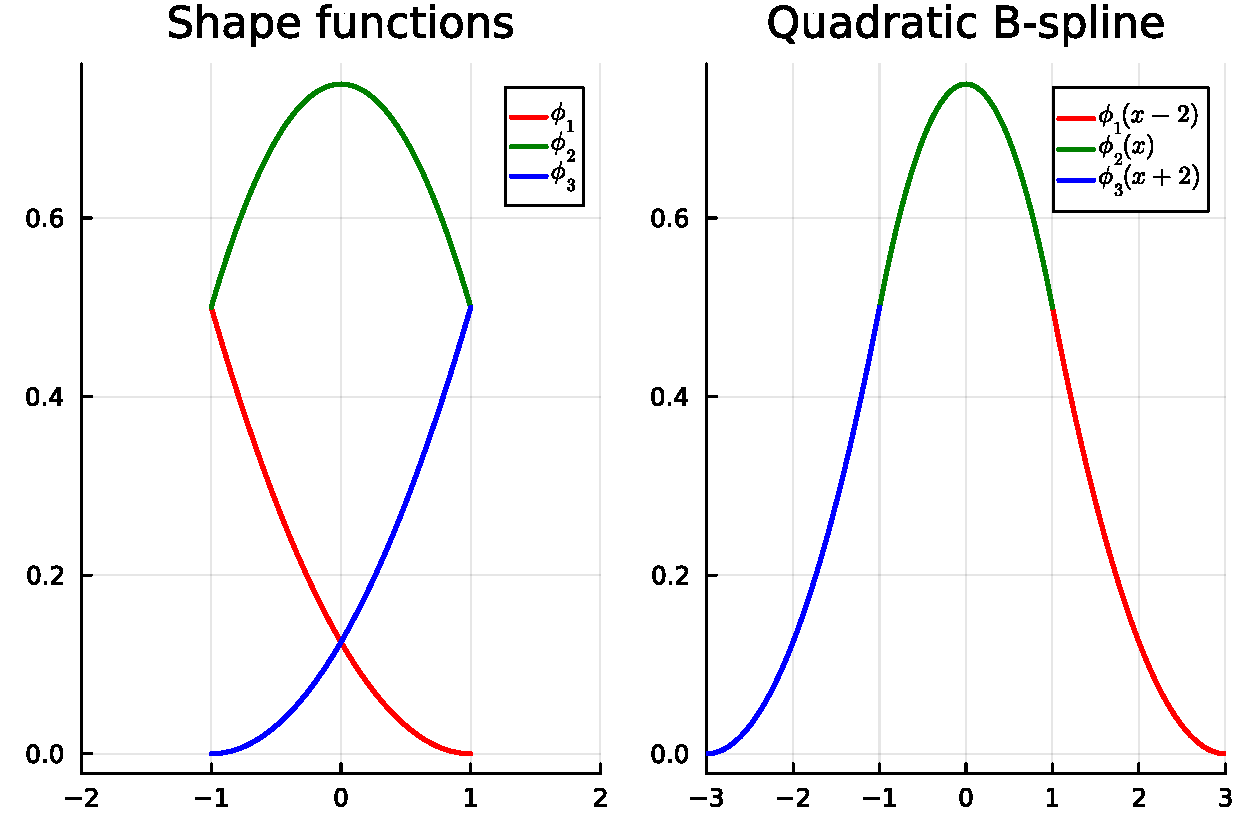
\includegraphics[width=\textwidth]{../../lectures/finite-elements/d-1/Bsplines/Bsplines_quadratic_shape.pdf}
        \end{column}
    \end{columns}
    \medskip
    \begin{itemize}
        \item Finite-element space: $\mathcal P_{\mathcal T} \cap C^1([a,b])$.
        \item Uniform meshes: $b_0 = \chi_{[0,1)}$, \ $b_p(x) = \int_{x-1}^x b_{p-1}(s)\diff s$ (support $[0,p+1]$), and
              \[
                  \mathcal P_{\mathcal T} \cap C^{p-1}([a,b]) = \Big\{ \sum_{i \in \mathbb Z} c_i\, b_p\big(\tfrac{x - x_i}{h}\big)\Big|_{(a,b)} \Big\}.
              \]
    \end{itemize}
\end{frame}

\begin{frame}{Clamped knots and cubic B-splines}
    \begin{columns}[T]
        \begin{column}{.48\textwidth}
            \centering
            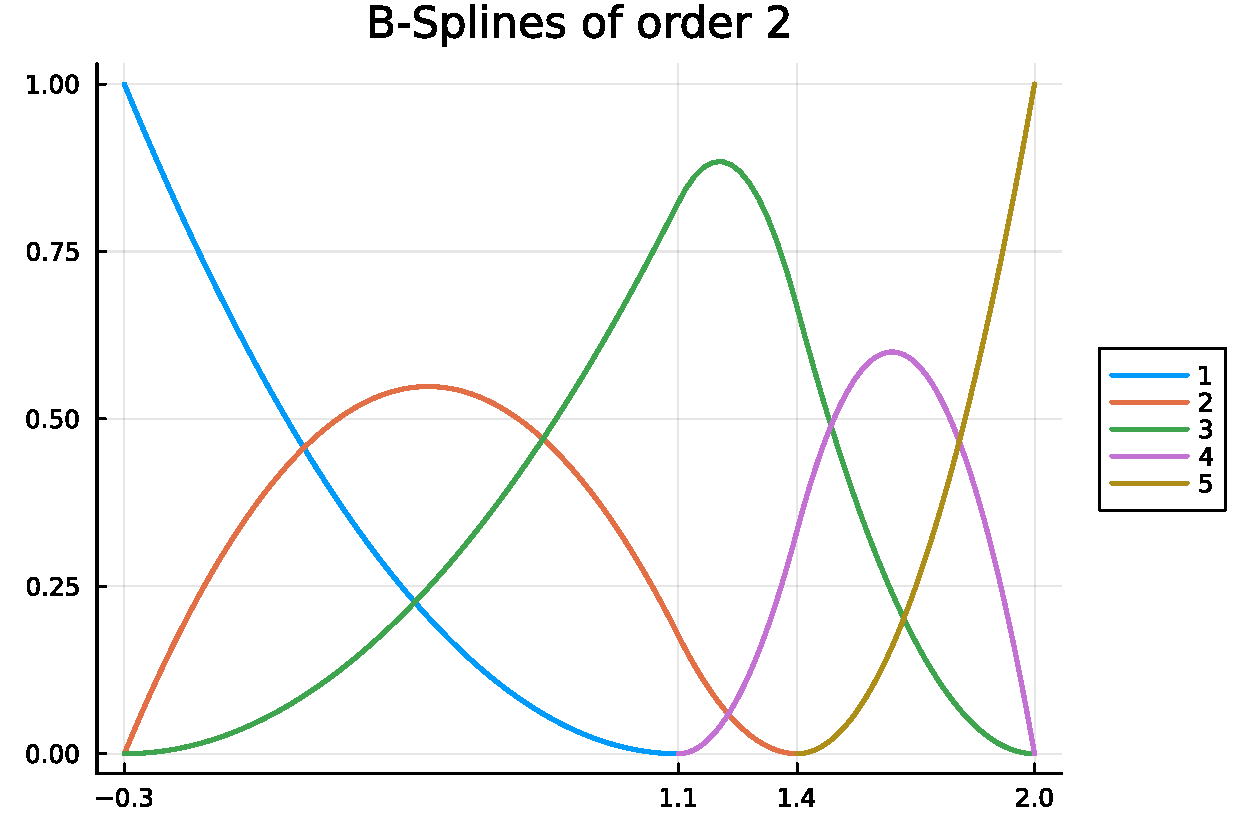
\includegraphics[width=.9\textwidth]{../../lectures/finite-elements/d-1/Bsplines/Bsplines_quadratic_basis.pdf}

            {\small Degree $2$: $\mathcal P_{\mathcal T} \cap C^1$}
        \end{column}
        \begin{column}{.48\textwidth}
            \centering
            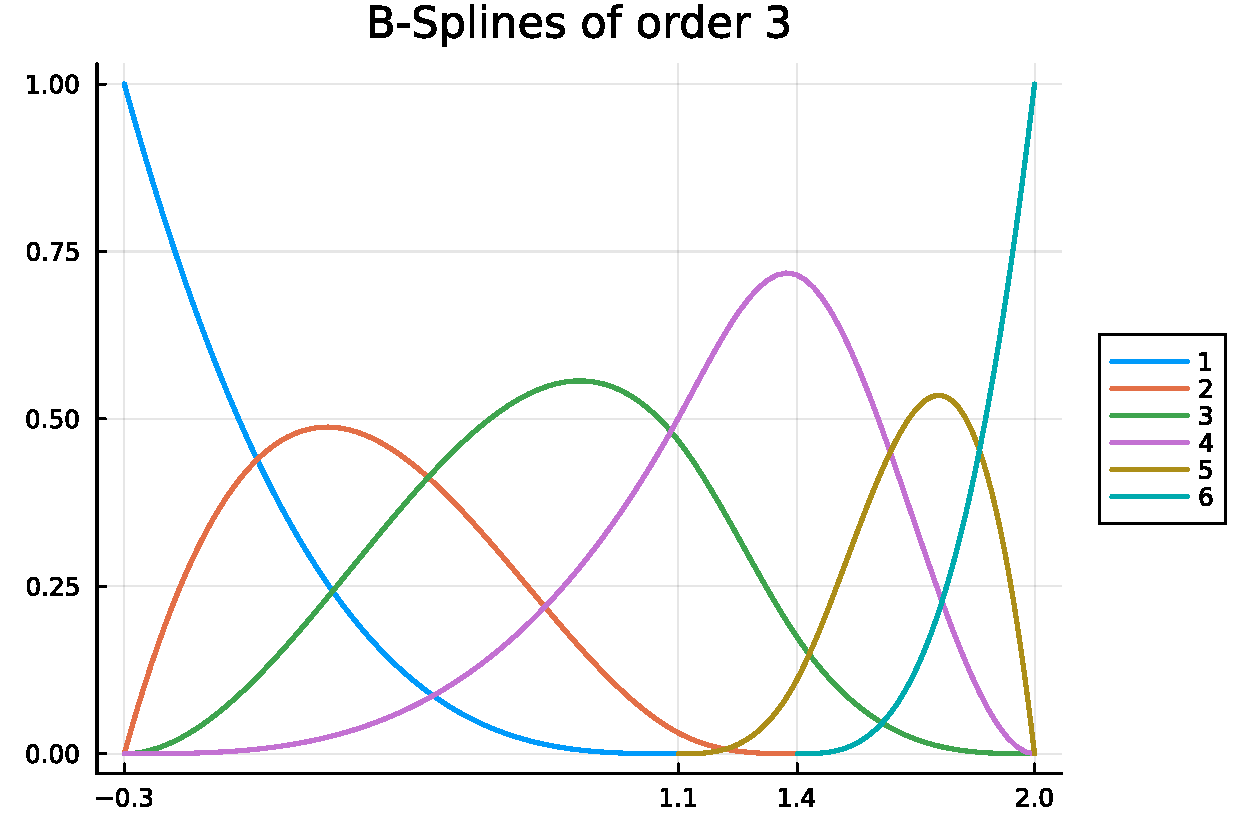
\includegraphics[width=.9\textwidth]{../../lectures/finite-elements/d-1/Bsplines/Bsplines_cubic_basis.pdf}

            {\small Degree $3$: $\mathcal P_{\mathcal T} \cap C^2$}
        \end{column}
    \end{columns}
    \medskip
    \begin{itemize}
        \item \alert{Clamped} knot vector: repeat each end point $p+1$ times (convention: terms with zero denominator are $0$).
        \item An interior knot of multiplicity $r$ reduces the continuity to $C^{p-r}$.
    \end{itemize}
\end{frame}

\begin{frame}{Summary and practice}
    \begin{itemize}
        \item Lagrange elements: $C^0$, high order for fixed degree.
        \item Hermite cubics: $C^1$ glueing, $\mathcal I_{\mathcal T}: H^2 \to H^2$, error $O(h^{4-j})$ in $H^j$.
        \item Implementation: reference matrices, local-to-global map, assembly loop over elements.
        \item B-splines: $C^{p-1}$ piece-wise polynomials of degree $p$ with minimal support.
    \end{itemize}
    \bigskip
    \textbf{Practice.}
    \begin{itemize}
        \item Notebooks \notebook{lectures/finite-elements/d-1/Hermite}{Hermite.ipynb} and \notebook{lectures/finite-elements/d-1/Bsplines}{Bsplines.ipynb}.
        \item Exercise 3.1: the beam equation $u'''' = f$ in $(-1,1)$.
              \board{weak formulation in $H^2$: $\int_{-1}^1 u'' v'' = \int_{-1}^1 f v$. Which boundary conditions go into $V$?}
    \end{itemize}
    \bigskip
    \textbf{Next session:} finite elements in $d = 2$.
\end{frame}
